\makeatletter\let\ifGm@compatii\relax\makeatother
\documentclass[xcolor=dvipsnames,ignorenonframetext]{beamer}
\usepackage{soul}
\def\Lnum{7}
\newcommand{\Pb}{\mathbb{P}}

\title[Intro to AI: Lecture \Lnum]{
  Probablities% \\[.5cm]
}


\author{Volker Sorge}


\date{}

\begin{document}
\only<article>{\addtocounter{page}{25}}
\begin{frame}
  \maketitle
\end{frame}
\tableofcontents

\section{Background}

\begin{frame}
  \frametitle{Uncertainty}
  \begin{itemize}
  \item So far we have assumed everything in our world is deterministic.
    \begin{itemize}
    \item If I use an umbrella, I will not get wet.
    \item What if the umbrella breaks in windy weather?
    \end{itemize}
  \end{itemize}
  \begin{itemize}
  \item Agent might need to act taking possible changes of the world into
    account.
  \item Agents needs to consider partial knowledge or events outside its own
    influence.
  \end{itemize}
\end{frame}


\begin{frame}
  \frametitle{Probabilistic Inference}
  \begin{itemize}
  \item Agents wants to learn about conditions in the world.
  \item Agents observes an event in the world.
  \item What where the likely causes of the event?
  \end{itemize}
\end{frame}

\section{Probability}

\begin{frame}
  \frametitle{Probability}
  \begin{itemize}
  \item \emph{Random Variable} $X$ describes the outcome of a \emph{stochastic
      event}.
  \item $X$ can take several values $\omega$, so called \emph{atomic events}.
  \item Values are drawn from a sample space $\Omega=\{\omega_1,\ldots,\omega_n\}$.
  \item Exactly one atomic event will happen.
  \item Atomic event or sample point tells us the complete state of the world,
    i.e., values of all random variables.
  \item Each atomic event has a probability $0 \leq P(X=\omega)\leq 1$
  \item Sum of all probabilities for all possible values of $X$ is $1$:
    \[\sum_{\omega\in\Omega}P(X=\omega)=1\]
  \item Probability distribution is
    $\Pb(X)=[P(X=\omega_1),P(X=\omega_2),\ldots,P(X=\omega_n)]$.
  \end{itemize}
\end{frame}

\begin{frame}
  \frametitle{Example: Probability}
  \begin{itemize}
  \item E.g., when rolling a die, the outcomes can be $X\in\{1,2,3,4,5,6\}$.
  \item $\Pb(X)=[\frac{1}{6}, \frac{1}{6}, \frac{1}{6}, \frac{1}{6}, \frac{1}{6}, \frac{1}{6}]$
  \item $P(X=4)=\frac{1}{6}$ or
  \item $P(X=1 \vee X=2)=P(X=1)+P(X=2)=\frac{2}{6}$ or
  \item $P(X<4)=P(X=1)+P(X=2)+P(X=3)=\frac{1}{2}$
  \end{itemize}
  If it is clear what random variable we are talking about we will omit the $X=$ part.
\end{frame}


\begin{frame}
  \frametitle{Multiple Random Variables}
  \begin{center}
    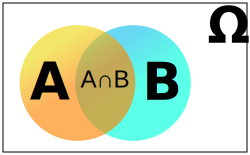
\includegraphics[width=.4\linewidth]{Probability_venn_a_b_intersection}
  \end{center}
  \begin{itemize}
  \item If events $A$ and $B$ are disjoint, then
    \[P(A \vee B) = P(A) + P(B)\]
  \item More generally:
    \[P(A \vee B) = P(A) + P(B) - P(A \wedge B)\]
  \item If events $A_1, \ldots, A_n$ are disjoint and exhaustive (one of them
    must happen) then $P(A_1) + ... + P(A_n) = 1$
  \end{itemize}
\end{frame}

\begin{frame}
  \frametitle{Combined Probabilities}
  \begin{itemize}
  \item If we have more than one random variable, we can compute \emph{joint probability distributions}.
  \item Let $X,Y$ be random variables, with possible values for
    $X\in\{x_1,\ldots,x_n\}, Y\in\{y_1,\ldots,y_m\}$.
    Then 
    \[\Pb(X,Y)=[\begin{array}[t]{lcl}
      P(X=x_1\wedge Y=y_1), & \ldots, & P(X=x_1\wedge Y=y_m) \\
      & \vdots &\\
      P(X=x_n\wedge Y=y_1), & \ldots, & P(X=x_n\wedge Y=y_m) ]
      \end{array}
      \]
  \item Marginalisation: 
    \[P(X=x)=\sum_y P(X=x\wedge Y=y)\]
    (Meaning sum over all possible atomic events $y$.)
  \end{itemize}
\end{frame}

\begin{frame}
  \frametitle{Example: Combined Probabilities}
  \begin{itemize}
  \item Roll two dice
  \item Random Variables:
    \begin{itemize}
    \item X = value of die 1
    \item Y = value of die 2
    \end{itemize}
  \item Outcome is represented by an ordered pair of values $(x, y)\in\{1,\ldots,6\}\times\{1,\ldots,6\}$.
  \item E.g., (6, 1): $P(X=6\wedge Y=1) = \frac{1}{36}$.
  \end{itemize}
  $\begin{array}{r|c|c|c|c|c|c}
    \textbf{$\Pb(X,Y)$} & \textbf{1} & \textbf{2} & \textbf{3} & \textbf{4} & \textbf{5} & \textbf{6}\\\hline
    \textbf{1} & \frac{1}{36} & \frac{1}{36} & \frac{1}{36} & \frac{1}{36} & \frac{1}{36}& \frac{1}{36}\\\hline
    \textbf{2} & \frac{1}{36} & \frac{1}{36} & \frac{1}{36} & \frac{1}{36} & \frac{1}{36}& \frac{1}{36}\\\hline
    \textbf{3} & \frac{1}{36} & \frac{1}{36} & \frac{1}{36} & \frac{1}{36} & \frac{1}{36}& \frac{1}{36}\\\hline
    \textbf{4} & \frac{1}{36} & \frac{1}{36} & \frac{1}{36} & \frac{1}{36} & \frac{1}{36}& \frac{1}{36}\\\hline
    \textbf{5} & \frac{1}{36} & \frac{1}{36} & \frac{1}{36} & \frac{1}{36} & \frac{1}{36}& \frac{1}{36}\\\hline
    \textbf{6} & \frac{1}{36} & \frac{1}{36} & \frac{1}{36} & \frac{1}{36} & \frac{1}{36}& \frac{1}{36}\\
  \end{array}$
\end{frame}

\section{Bayes Rule}

\begin{frame}
  \frametitle{Conditional Probability} 

  Consider a game of Poker: Given that your
  first two cards are Queens, what is the probability that you will get at least
  3 Queens?

  \begin{itemize}
  \item Conditional probability 
    \[P(X|Y)\]
  \item What is the probability that $X$ happens when $Y$ happens?
  \item Or: $X | Y$ is true in the fraction of worlds where $X\wedge Y$ is true
    out of the total possible worlds where $X$ is true.
  \end{itemize}
\end{frame}

\begin{frame}
  \frametitle{Bayes' Rule}
  \begin{center}
    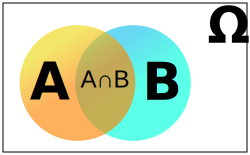
\includegraphics[width=.4\linewidth]{Probability_venn_a_b_intersection}
  \end{center}
  \begin{equation}
    \label{eq:bayes1}
    P(A|B)=\frac{P(A\wedge B)}{P(B)}
  \end{equation}
  This implies
  \begin{eqnarray}
    \label{eq:bayes2}
    P(A|B)P(B)=P(A\wedge B)  
  \end{eqnarray}
  \begin{eqnarray}
    \label{eq:bayes3}
    P(A|B)=\frac{P(B|A)P(A)}{P(B)}
  \end{eqnarray}
\end{frame}

\begin{frame}
  \frametitle{Example: Conditional Probability} 
  \begin{tabular}{c|c|c}
    & Raining & $\neg$Raining \\\hline
    Sprinklers & $.12$ & $.28$ \\\hline
    $\neg$Sprinklers & $.18$ & $.42$ 
  \end{tabular}

  \begin{itemize}
  \item It is raining and the sprinklers are on? \\
    \centerline{$P(\mathrm{Raining} \wedge \mathrm{Sprinklers})=.12$}
  \item It is raining?\\
    \centerline{$P(\mathrm{Raining}) = .12 + .18 = .3$}
  \item Sprinklers on, given that it is not raining?\\
    \centerline{$P(\mathrm{Sprinklers}|\neg\mathrm{Raining})= \frac{.28}{.7}= .4$}
  \end{itemize}
\end{frame}

\begin{frame}
  \frametitle{Probabilistic Evidence}
  \begin{itemize}
  \item Suppose we already know an event in our world.
  \item What evidence is there for a particular cause of that event?
  \item I.e., compute $P(X|X\wedge Y)$.
  \end{itemize}
\end{frame}

\begin{frame}
  \frametitle{Example: Conditional Probability}
  \begin{itemize}
  \item Suppose we know that $X+Y=6$ or $X+Y=7$.
  \item What is the probability of $Y=5$?
  \item Part of the sample space is eliminated; probabilities are renormalised to sum to 1.
  \end{itemize}

  {\small\arraycolsep4pt
    $\begin{array}{r|c|c|c|c|c|c}
    & \textbf{1} & \textbf{2} & \textbf{3} & \textbf{4} & \textbf{5} & \textbf{6}\\\hline
    \textbf{1} & \frac{1}{36} & \frac{1}{36} & \frac{1}{36} & \frac{1}{36} & \frac{1}{36}& \frac{1}{36}\\\hline
    \textbf{2} & \frac{1}{36} & \frac{1}{36} & \frac{1}{36} & \frac{1}{36} & \frac{1}{36}& \frac{1}{36}\\\hline
    \textbf{3} & \frac{1}{36} & \frac{1}{36} & \frac{1}{36} & \frac{1}{36} & \frac{1}{36}& \frac{1}{36}\\\hline
    \textbf{4} & \frac{1}{36} & \frac{1}{36} & \frac{1}{36} & \frac{1}{36} & \frac{1}{36}& \frac{1}{36}\\\hline
    \textbf{5} & \frac{1}{36} & \frac{1}{36} & \frac{1}{36} & \frac{1}{36} & \frac{1}{36}& \frac{1}{36}\\\hline
    \textbf{6} & \frac{1}{36} & \frac{1}{36} & \frac{1}{36} & \frac{1}{36} & \frac{1}{36}& \frac{1}{36}\\
  \end{array}\rightarrow
  \begin{array}{r|c|c|c|c|c|c}
    & \textbf{1} & \textbf{2} & \textbf{3} & \textbf{4} & \textbf{5} & \textbf{6}\\\hline
    \textbf{1} & 0 & 0 & 0 & 0 & \frac{1}{11}& \frac{1}{11}\\
    \textbf{2} & 0 & 0 & 0 & \frac{1}{11} & \frac{1}{11}& 0\\\hline
    \textbf{3} & 0 & 0 & \frac{1}{11} & \frac{1}{11} & 0& 0\\\hline
    \textbf{4} & 0 & \frac{1}{11} & \frac{1}{11} & 0 & 0& 0\\\hline
    \textbf{5} & \frac{1}{11} & \frac{1}{11} & 0 & 0 & 0& 0\\\hline
    \textbf{6} & \frac{1}{11} & 0 & 0 & 0 & 0& 0\\\hline
  \end{array}$}
  \begin{itemize}
  \item $P(Y=5|(X+Y=6)\vee(X+Y=7))=\frac{2}{11}$.
  \end{itemize}
\end{frame}

\begin{frame}
  \frametitle{Probabilistic Reasoning}
  \begin{itemize}
  \item We have now a complete approach for reasoning under uncertainty:
    \begin{enumerate}
    \item Specify probability for every atomic event,
    \item Compute probabilities of events simply by summing
      probabilities of atomic events,
    \item Conditional probabilities are specified in terms of
      probabilities of events: $P(A | B) = \frac{P(A \wedge B)}{P(B)}$.
    \end{enumerate}
  \end{itemize}
  Does that scale?
  \begin{itemize}
  \item $n$ variables that can each take $k$ values.
  \item What is the number of atomic events?
  \end{itemize}
\end{frame}

\section{Independence}

\begin{frame}
  \frametitle{Independence}
  \begin{itemize}
  \item Some variables are independent.
  \item For example, the roll of two dice have nothing to do with each other.
  \item In other words: the outcome of random variable $X$ does not tell us
    anything about $Y$.
  \item Hence $P(Y=y|X=x)=P(Y=y)$ and $P(X=x|Y=y)=P(X=x)$ 
  \item Thus we can compute $P(X\wedge Y) = P(X)P(Y)$.
  \end{itemize}
\end{frame}

\begin{frame}
  \frametitle{Conditional Independence}
  \begin{itemize}
  \item Intuition:
    \begin{itemize}
    \item the only reason that X told us something about Y,
    \item is that X told us something about Z,
    \item and Z tells us something about Y
    \end{itemize}
  \item If we already know Z, then X tells us nothing about Y.
  \item $P(Y | Z\wedge X) = P(Y | Z)$ or
  \item $P(X\wedge Y | Z) = P(X | Z)P(Y | Z)$
  \item Meaning:\newline  "X and Y are conditionally independent given Z"
  \end{itemize}
\end{frame}

\begin{frame}
  \frametitle{Example: Rigged Casino}
    \begin{itemize}
    \item With probability $\frac{1}{2}$, the casino is rigged and has dice that
      come up $6$ only $\frac{1}{12}$ of the time, and $1$ $\frac{3}{12}$ of the
      time.
  \end{itemize}
  {\small\arraycolsep4pt
    $\begin{array}{r|c|c|c|c|c|c}
      \multicolumn{7}{c}{\neg Z \text{ (fair casino)}}\\
    & \textbf{1} & \textbf{2} & \textbf{3} & \textbf{4} & \textbf{5} & \textbf{6}\\\hline
    \textbf{1} & \frac{1}{72} & \frac{1}{72} & \frac{1}{72} & \frac{1}{72} & \frac{1}{72}& \frac{1}{72}\\\hline
    \textbf{2} & \frac{1}{72} & \frac{1}{72} & \frac{1}{72} & \frac{1}{72} & \frac{1}{72}& \frac{1}{72}\\\hline
    \textbf{3} & \frac{1}{72} & \frac{1}{72} & \frac{1}{72} & \frac{1}{72} & \frac{1}{72}& \frac{1}{72}\\\hline
    \textbf{4} & \frac{1}{72} & \frac{1}{72} & \frac{1}{72} & \frac{1}{72} & \frac{1}{72}& \frac{1}{72}\\\hline
    \textbf{5} & \frac{1}{72} & \frac{1}{72} & \frac{1}{72} & \frac{1}{72} & \frac{1}{72}& \frac{1}{72}\\\hline
    \textbf{6} & \frac{1}{72} & \frac{1}{72} & \frac{1}{72} & \frac{1}{72} & \frac{1}{72}& \frac{1}{72}\\
  \end{array}\rightarrow
  \begin{array}{r|c|c|c|c|c|c}
    \multicolumn{7}{c}{Z \text{ (rigged casino)}}\\
    & \textbf{1} & \textbf{2} & \textbf{3} & \textbf{4} & \textbf{5} & \textbf{6}\\\hline
    \textbf{1} & \frac{1}{32} & \frac{1}{48} & \frac{1}{48} & \frac{1}{48} & \frac{1}{48}& \frac{1}{96}\\\hline
    \textbf{2} & \frac{1}{48} & \frac{1}{72} & \frac{1}{72} & \frac{1}{72} & \frac{1}{72}& \frac{1}{144}\\\hline
    \textbf{3} & \frac{1}{48} & \frac{1}{72} & \frac{1}{72} & \frac{1}{72} & \frac{1}{72}& \frac{1}{144}\\\hline
    \textbf{4} & \frac{1}{48} & \frac{1}{72} & \frac{1}{72} & \frac{1}{72} & \frac{1}{72}& \frac{1}{144}\\\hline
    \textbf{5} & \frac{1}{48} & \frac{1}{72} & \frac{1}{72} & \frac{1}{72} & \frac{1}{72}& \frac{1}{144}\\\hline
    \textbf{6} & \frac{1}{96} & \frac{1}{144} & \frac{1}{144} & \frac{1}{144} & \frac{1}{144}& \frac{1}{288}\\
  \end{array}$}
  \begin{itemize}
  \item What is $P(Y=6)$?
  \item What is $P(Y=6|X=1)$?
  \item Are they independent?
  \end{itemize}
\end{frame}


\begin{frame}
  \frametitle{Independence vs Dependence}
  \begin{itemize}
  \item Suppose both Mark and Volker both start work in the department at 9am.
  \item What is the probability that
    \begin{itemize}
    \item Mark is late today?
    \item Volker is late today?
    \end{itemize}
  \item Clearly those events are independent.
  \end{itemize}
  Now consider the following information:
  \begin{itemize}
  \item Both Mark and Volker live in Kings Heath.
  \item Now we can construct a dependency between the two.
  \item For example, if we learn that the Pershore is closed, then Mark arriving
    late could imply Volker arriving late as well.
  \end{itemize}
\end{frame}

\begin{frame}
  \frametitle{A More Formal Example}
  \begin{itemize}
  \item Let's define the following three random variables:
    \begin{itemize}
    \item X: Lecturer A arrives late.
    \item Y: Lecturer B arrives late.
    \item Z: Lecturer A and B live in the same suburb.
    \end{itemize}
  \item As soon we know whether or not $Z$ holds, $X$ and $Y$ are independent
    again.
  \end{itemize}
  \begin{itemize}
  \item Suppose we know the following probabilities
    \begin{itemize}
    \item $P(Z)=.2$
    \item $P(X|Z) = .5$ and $P(X|\neg Z)=.2$
    \item $P(Y|Z) = .4$ and $P(Y|\neg Z)=.1$
    \end{itemize}
  \item Can we compute $P(Z|X)$ or $P(Z|X\wedge \neg Y)$?
  \end{itemize}
\end{frame}



\begin{frame}
  \frametitle{Conditioning}
  \begin{description}
  \item[Marginalisation] is effectively summing out a random variable:
    \begin{equation}
      \label{eq:marginalisation}
      P(X)=\sum_y P(X\wedge y)  
    \end{equation}
  \item[Conditioning] with \hyperref[eq:bayes2]{Bayes~(\ref{eq:bayes2})} and
    \hyperref[eq:marginalisation]{marginalisation~(\ref{eq:marginalisation})}:
    \begin{equation}
      \label{eq:new1}
      P(X)=\sum_y P(X|y) P(y)
    \end{equation}
    (Again we sum over all values $y$ for $Y$.)
  \end{description}
\end{frame}


\begin{frame}
  \frametitle{Normalisation}
  \begin{description}
  \item[Normalisation] with \hyperref[eq:bayes1]{Bayes~(\ref{eq:bayes1})}
    \begin{equation}
      \label{eq:new3}
      P(X|Y)=\frac{P(X\wedge Y)}{P(Y)}=\alpha P(X\wedge Y)
    \end{equation}
  \end{description}
  $\alpha$ is the normalisation constant. It can be computed by normalising
  the probability distribution $\Pb(X|Y=y)$ for some value $y$ of $Y$, to add
  up to $1$, thus eliminating the need for $P(Y)$.
\end{frame}
  
\begin{frame}
  \frametitle{Normalisation Application}
  \begin{itemize}
  \item 
    Normalisation is used to compute evidence for a query.
  \item Let $X, E, Y$ be random variables. ($E,Y$ can be sets of variables.) Then we say
    \begin{itemize}
    \item $X$ is the query variable,
    \item $E$ is the evidence variable, and $e$ an observed value for $E$,
    \item $Y$ is the unobserved variable. 
    \end{itemize}
  \item Evidence for $X$ under observation $e$ is computed as:
  \end{itemize}
    \[ \Pb(X|e) = \alpha\Pb(X, e)=\alpha\sum_y \Pb(X, e, y)\]
    Again we sum over all possible values $y$ for $Y$.
\end{frame}


\begin{frame}
  \frametitle{Example: Full Joint Distribution}
  X: is it raining?, Y: are sprinklers on?, Z: is the grass wet?
  \begin{center}
    $\begin{array}{|r|c|c|c|c|} \hline
& \multicolumn{2}{c|}{\neg \mathrm{Wet}} &
      \multicolumn{2}{c|}{\mathrm{Wet}}\\\cline{2-5}
      & \mathrm{Rain} & \neg \mathrm{Rain} & \mathrm{Rain} & \neg \mathrm{Rain}\\\hline
      \mathrm{Sprinkler} & .012 & .056 & .108 & .224 \\\hline
      \neg \mathrm{Sprinkler} & .054 & .378 & .126 & .042 \\\hline
    \end{array}$
  \end{center}
  \begin{itemize}
  \item How likely is the grass wet when it rains?
    \onslide<2>{{\small \begin{eqnarray*}
      P(Z|X=\mathrm{Rain}) & = & \alpha\Pb(Z,r) \\
      &= &
      \alpha [ \Pb(Z, r, s) + \Pb(Z, r,\neg s)]\\
      & = & \alpha[ \langle P(w\wedge r\wedge s), P(\neg w\wedge r\wedge s)\rangle\\
      & & \quad + \langle P(w\wedge r\wedge \neg s), P(\neg w\wedge r\wedge \neg s)\rangle]\\
      & = & \alpha[ \langle.108, .012\rangle + \langle.126, .054\rangle]\\
      & = & \alpha[ \langle.234, .066\rangle]\\
      & = & [ \langle.78, .22\rangle] \text{\qquad\qquad with } \alpha=\frac{1}{.3}\\
    \end{eqnarray*}}
  Hence $P(\mathrm{Wet}|\mathrm{Rain})= .78$}
  \end{itemize}
\end{frame}


\begin{frame}
  \frametitle{Consequences of Bayes' Rule}
  \begin{description}
  \item[Adding Evidence] with \hyperref[eq:bayes3]{Bayes~(\ref{eq:bayes3})} and
    some evidence value $e$:
    \begin{equation}
      \label{eq:new2}
      \Pb(Y|X, e) = \frac{\Pb(X|Y, e)\Pb(Y|e)}{\Pb(X|e)}
    \end{equation}
  \item[Absolute Independence]
    \begin{eqnarray}
 \Pb(X, Y) & = &  \Pb(X) \Pb(Y)\\
 \Pb(X| Y) & = &  \Pb(X)\\
 \Pb(Y| X) & = &  \Pb(Y)
    \end{eqnarray}
  \item[Conditional Independence] 
    \begin{eqnarray}
 \Pb(X, Y | Z) & = &  \Pb(X | Z) \Pb(Y | Z)\\
 \Pb(X | Y, Z) & = &  \Pb(X | Z)\\
 \Pb(Y | X, Z) & = &  \Pb(Y | Z)
    \end{eqnarray}
  \end{description}
\end{frame}


\end{document}


%%% Local Variables: 
%%% mode: latex
%%% TeX-master: t
%%% End: 


